%
% fxy.tex
%
% (c) 2021 Prof Dr Andreas Müller, OST Ostschweizer Fachhochschule
%
\documentclass[tikz]{standalone}
\usepackage{times}
\usepackage{amsmath}
\usepackage{txfonts}
\usepackage[utf8]{inputenc}
\usepackage{graphics}
\usetikzlibrary{arrows,intersections,math}
\usepackage{ifthen}
\begin{document}

\definecolor{darkgreen}{rgb}{0,0.6,0}
\definecolor{rosa}{rgb}{0.8,0.4,0.8}

\newboolean{showgrid}
\setboolean{showgrid}{false}
\def\breite{7}
\def\hoehe{4}

\begin{tikzpicture}[>=latex,thick]
\clip (-6.3,-3.2) rectangle (6.3,2.3);

% Povray Bild
\node at (-3.15,0) {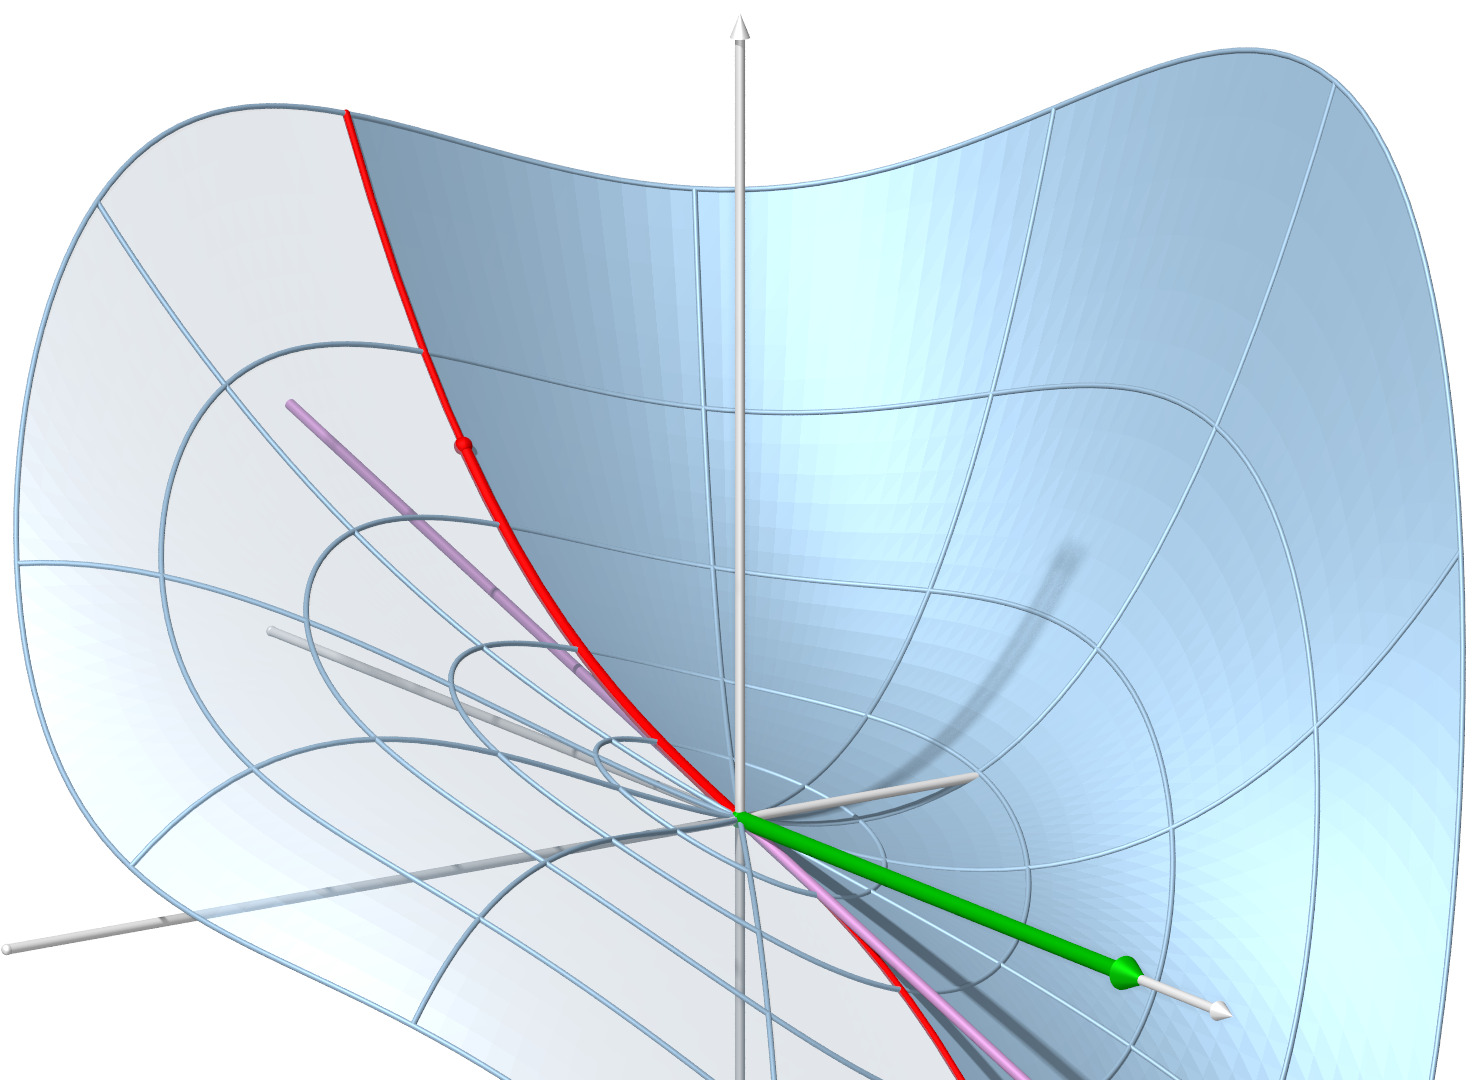
\includegraphics[width=6.3cm]{fx.jpg}};
\node at (3.15,0) {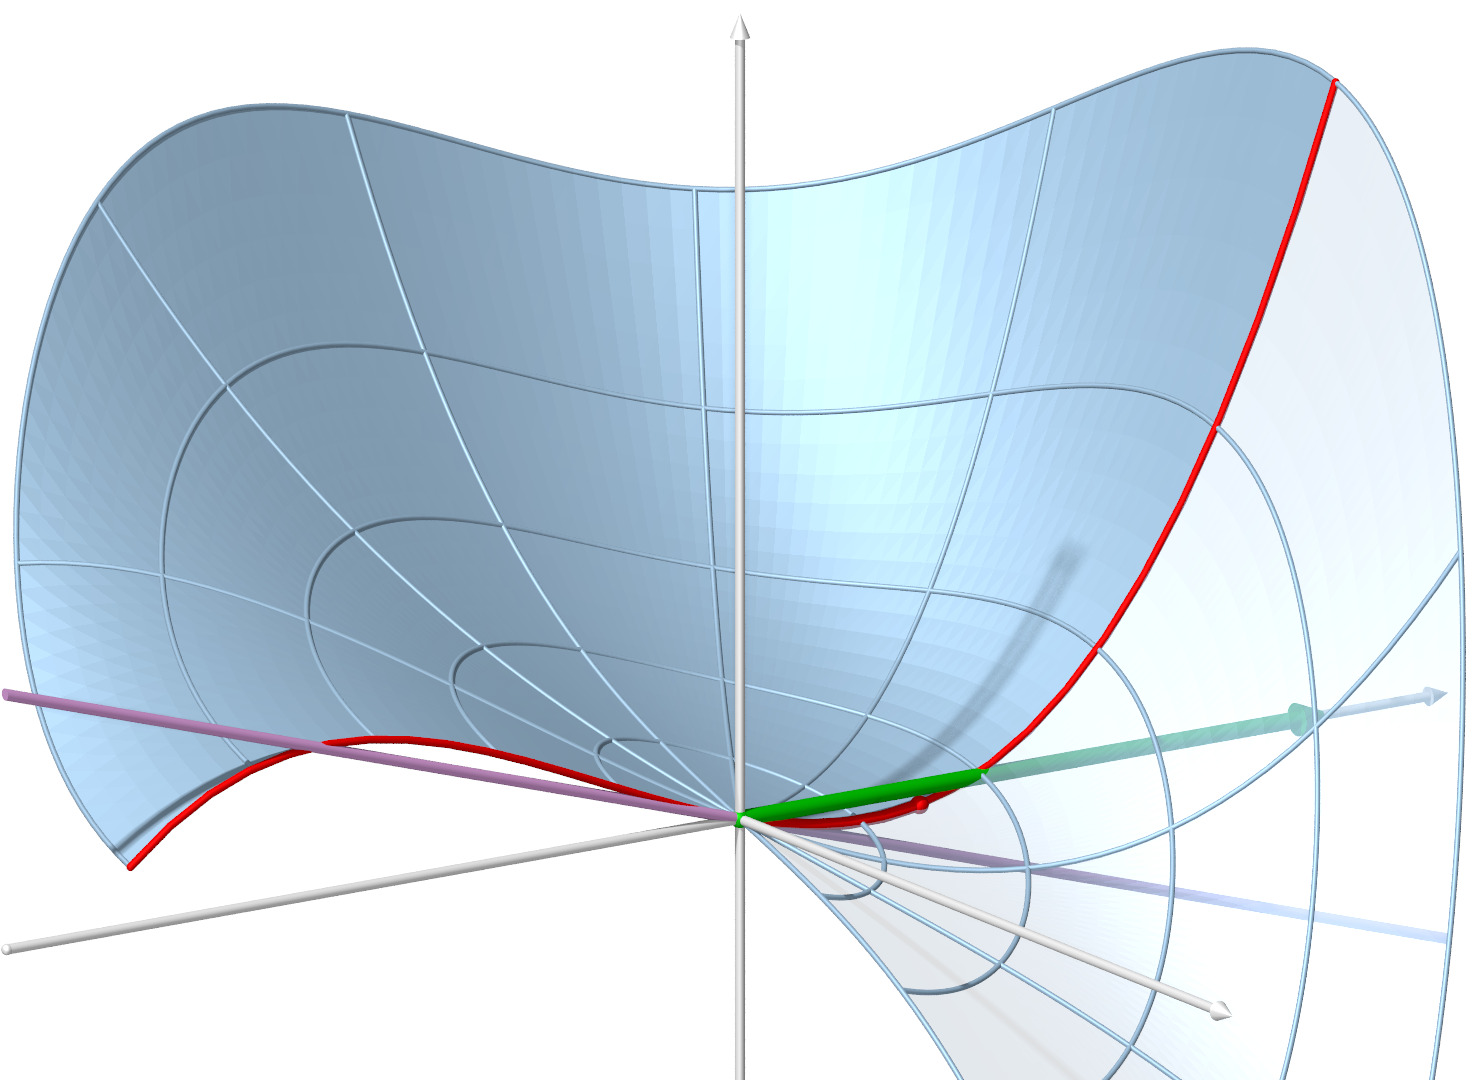
\includegraphics[width=6.3cm]{fy.jpg}};

% Gitter
\ifthenelse{\boolean{showgrid}}{
\draw[step=0.1,line width=0.1pt] (-\breite,-\hoehe) grid (\breite, \hoehe);
\draw[step=0.5,line width=0.4pt] (-\breite,-\hoehe) grid (\breite, \hoehe);
\draw                            (-\breite,-\hoehe) grid (\breite, \hoehe);
\fill (0,0) circle[radius=0.05];
}{}

\node at (-0.9,-1.9) {$x\mathstrut$};
\node at (-6,-1.9) {$-y\mathstrut$};
\node at (-3.4,2.2) {$z\mathstrut$};
\node[color=white] at (-1.3,1.5) {$z=f(x,y)\mathstrut$};
\node[color=darkgreen] at (-1.4,-1.6) {$\vec{e}_1$};
\node[color=rosa] at (-2.2,-2.3) [below right]
	{$\displaystyle\frac{\partial f}{\partial x}={\color{darkgreen}D_{\vec{e}_1}}f$};

\node at (5.4,-1.9) {$x\mathstrut$};
\node at (6.1,-0.5) {$y\mathstrut$};
\node at (3,2.2) {$z\mathstrut$};
\node[color=white] at (4.7,1.5) {$z=f(x,y)\mathstrut$};
\node[color=darkgreen] at (5.6,-0.5) {$\vec{e}_2$};
\node[color=rosa] at (1,-0.9) [below right]
	{$\displaystyle\frac{\partial f}{\partial y}={\color{darkgreen}D_{\vec{e}_2}}f$};

\end{tikzpicture}

\end{document}

